\chapter{Обобщенная модель Изинга на квадратной решетке при учете декорирования}\label{ch:ch6}


\section{Точное решение обобщенной модели Изинга на квадратной решетке с учетом декорирования}

На рисунке~\ref{squareDecor} продемонстрирована квадратная решетка с двумя трансляциями при учете декорирования. Как и в Главе~\ref{ch:ch3}, нодальные спины представлены черными кружками, а декорированные --- синими. 

 \begin{figure}[h]
	\center{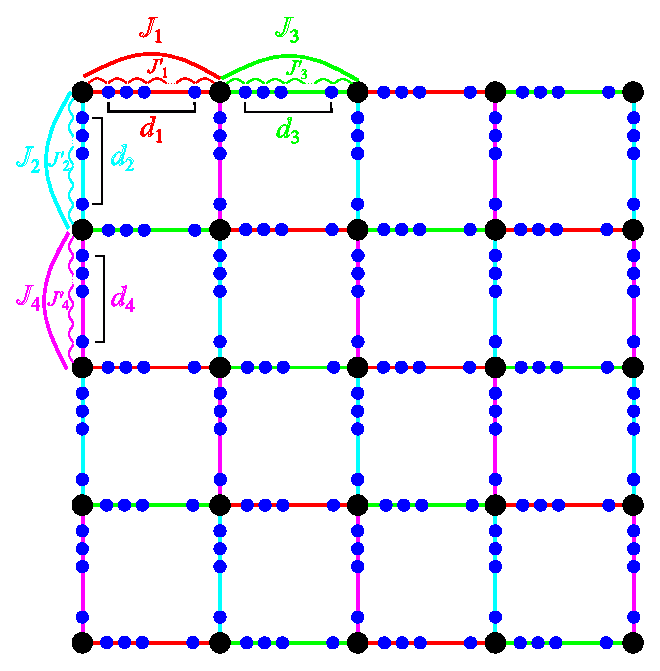
\includegraphics[width=0.55\linewidth]{part6/genDecorLattice.eps}}
	\caption{Квадратная решетка с двумя трансляциями при учете декорирования}
	\label{squareDecor}
\end{figure}

Поскольку рассматривается декорированная квадратная решетка с обобщением на две трансляции решетки, то задача имеет 8 параметров обменного взаимодействия, включая 4 параметра между нодальными спинами $J_1, J_2, J_3, J_4$ и 4 параметра между декорированными и нодальными и между только нодальными спинами $J_{d_1}, J_{d_2}, J_{d_3}, J_{d_4}$, которые можно варьировать не только по величине, но и по знаку. Вдобавок, имеются 4 степени декорирования: $d_1, d_3$ -- по горизонтали, $d_2, d_4$ -- по вертикали, которые также можно изменять по величине. 


\section{Спонтанная намагниченность обобщенной модели Изинга на квадратной решетке с учетом декорирования}



\section{Термодинамические, фрустрационные особенности обобщенной модели Изинга на квадратной решетке при учете декорирования}

Задавая параметры обменного взаимодействия как $J_1 = -1, J_2 = -1, J_3 = -1, J_4 = -1, J_{d_1} = 1, J_{d_2} = 1, J_{d_3} = 1, J_{d_4} = 1$, а степени декорирования --- $d_1 = 2, d_2 = 2, d_3 = 1, d_4 = 1$, получается фрустрированное состояние рассматриваемой модели Изинга, поскольку вместо узкого онзагеровского пика теплоемкости получается широкий пик (рис.~\ref{0trans}а), а энтропия при стремлении температуры к нулю отлична от нуля (рис.~\ref{0trans}б). В результате, при таких заданных параметрах система не претерпевает ни одного фазового перехода.

 \begin{figure}[h]
	\begin{minipage}{0.47\linewidth}
		\center{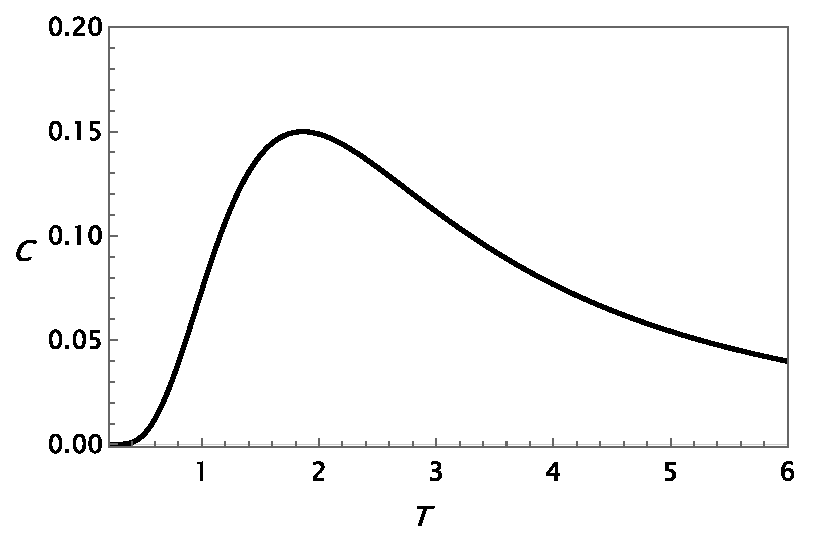
\includegraphics[width=1\linewidth]{part6/0transCap.eps} \\ а)}
	\end{minipage}
	\hfill
	\begin{minipage}{0.47\linewidth}
		\center{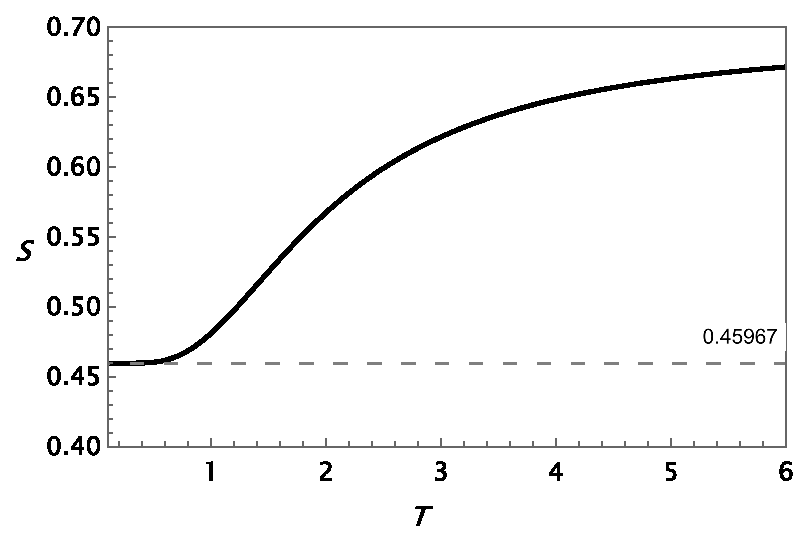
\includegraphics[width=1\linewidth]{part6/0transEnt.eps} \\ б)}
	\end{minipage}
	\caption{а) Теплоемкость и б) энтропия как функции температуры при $J_1 = -1, J_2 = -1, J_3 = -1, J_4 = -1, J_{d_1} = 1, J_{d_2} = 1, J_{d_3} = 1, J_{d_4} = 1$ и $d_1 = 2, d_2 = 2, d_3 = 1, d_4 = 1$}
	\label{0trans}
\end{figure}

Теперь, если выбрать параметры обменного взаимодействия как $J_1 = -1, J_2 = -1, J_3 = -1, J_4 = -1, J_{d_1} = 1, J_{d_2} = 1, J_{d_3} = 1, J_{d_4} = 1$ при степенях декорирования $d_1 = 2, d_2 = 3, d_3 = 1, d_4 = 3$, то в системе будет фазовый переход. На рисунке~\ref{1trans}а проиллюстрирована теплоемкость как функция температуры со значением температуры фазового перехода $T_N \approx 1.66$. Энтропия при этом не равна нулю при стремлении температуры к нулю (рис.~\ref{1trans}б). Спонтанная намагниченность, показанная на рисунке~\ref{1trans}, имеет совершенно классический вид для системы "антиферромагнетик -- парамагнетик". При низких температурах система обладает максимальной упорядоченностью спинов, что символизирует равенство спонтанной намагниченности единице при $T \rightarrow 0$. Затем при увеличении температуры начинает происходить разупорядочение спинов и в при некоторой температуре перехода $T_N$ спонтанная намагниченность в системе исчезает полностью. Дальнейшее увеличение температуры ни на что не повлияет, система уже и так полностью разупорядочена, а ее энтропия (на один узел решетки) равна $\ln 2$.  

 \begin{figure}[h]
	\begin{minipage}{0.47\linewidth}
		\center{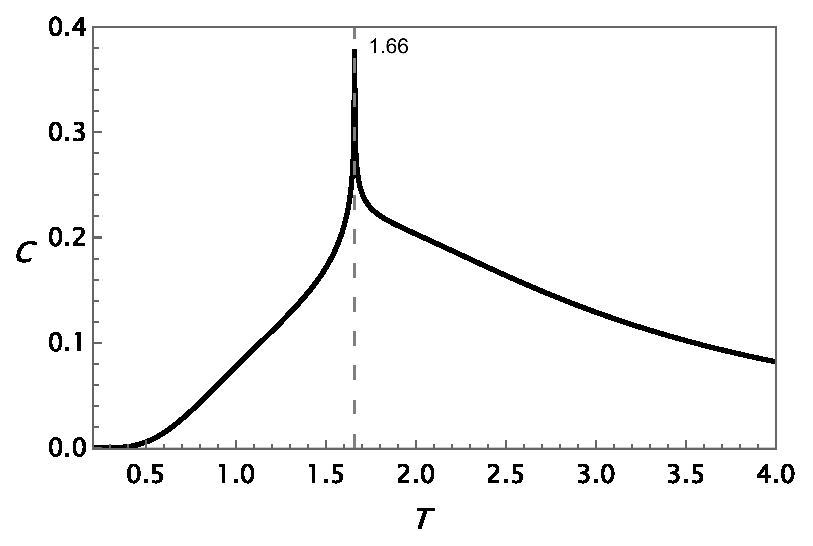
\includegraphics[width=1\linewidth]{part6/1transCap.eps} \\ а)}
	\end{minipage}
	\hfill
	\begin{minipage}{0.47\linewidth}
		\center{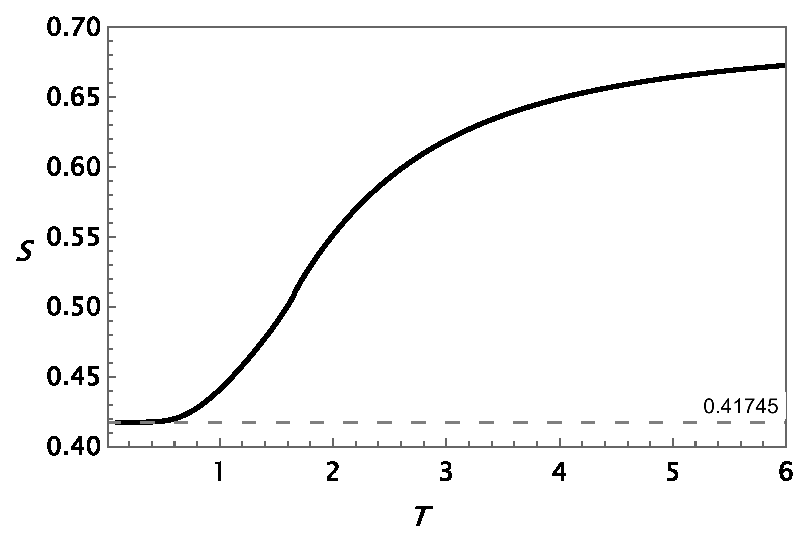
\includegraphics[width=1\linewidth]{part6/1transEnt.eps} \\ б)}
	\end{minipage}
	\vfill
	\begin{minipage}{0.47\linewidth}
		\center{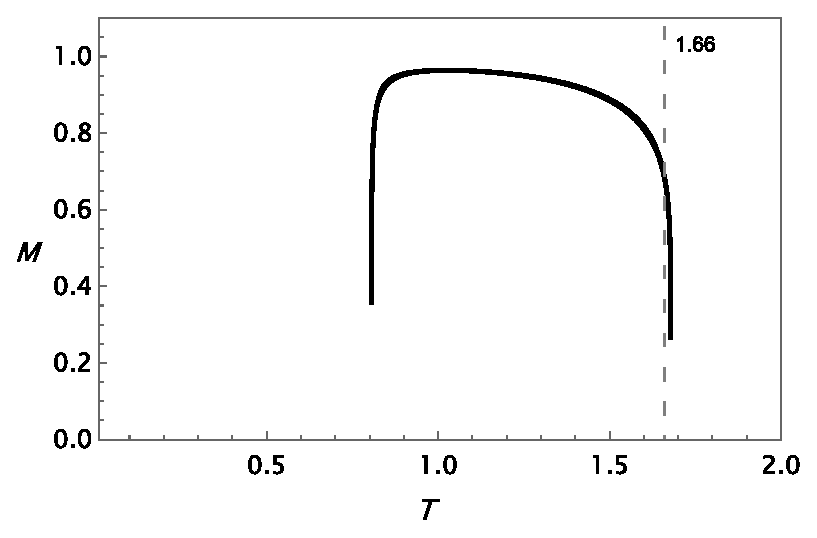
\includegraphics[width=1\linewidth]{part6/1transMag.eps} \\ в)}
	\end{minipage}
	\caption{а) Теплоемкость; б) энтропия и в) спонтанная намагниченность как функции температуры при $J_1 = -1, J_2 = -1, J_3 = -1, J_4 = -1, J_{d_1} = 1, J_{d_2} = 1, J_{d_3} = 1, J_{d_4} = 1$ и $d_1 = 2, d_2 = 3, d_3 = 1, d_4 = 3$}
	\label{1trans}
\end{figure}

Изменив параметры обменного взаимодействия как $J_1 = 0.1, J_2 = -1.3, J_3 = -1.3, J_4 = -1.3, J_{d_1} = 1, J_{d_2} = 1, J_{d_3} = 1, J_{d_4} = 1$ со степенями декорирования $d_1 = 4, d_2 = 4, d_3 = 4, d_4 = 4$, получается уже два фазовых перехода. Об этом свидетельствуют рисунки теплоемкости~(рис.~\ref{2trans}а), энтропии~(рис.~\ref{2trans}б) и спонтанной намагниченности~(рис.~\ref{2trans}в). На рисунке~\ref{2trans}в в интервале температур от $T = 0$ до некоторой температуры перехода $T_{N_1}$ спонтанная намагниченность сначала отсутствует. Только начиная от $T_{N_1} \approx 0.80598$ и далее она начинает повышаться до насыщения, после чего снова идет на спад, и уже при $T_N \approx 1.6781$ становится равной нулю. 

 \begin{figure}[h]
	\begin{minipage}{0.47\linewidth}
		\center{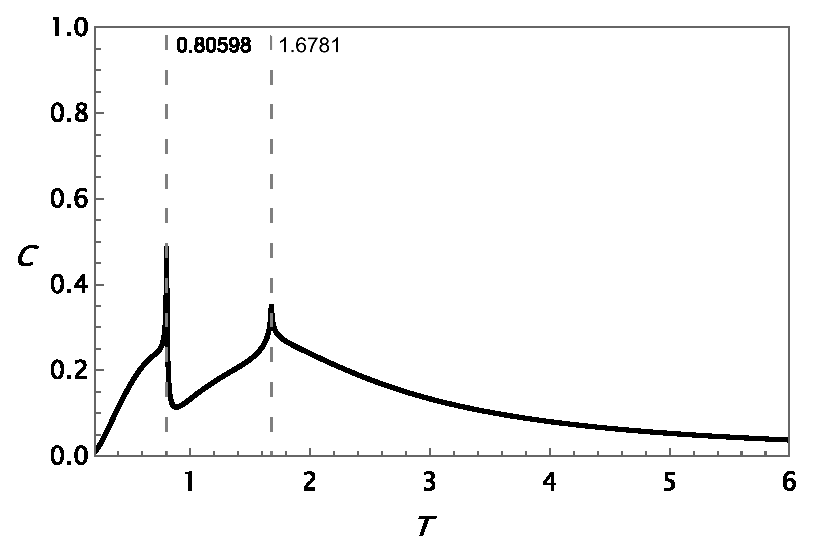
\includegraphics[width=1\linewidth]{part6/2transCap2.eps} \\ а)}
	\end{minipage}
	\hfill
	\begin{minipage}{0.47\linewidth}
		\center{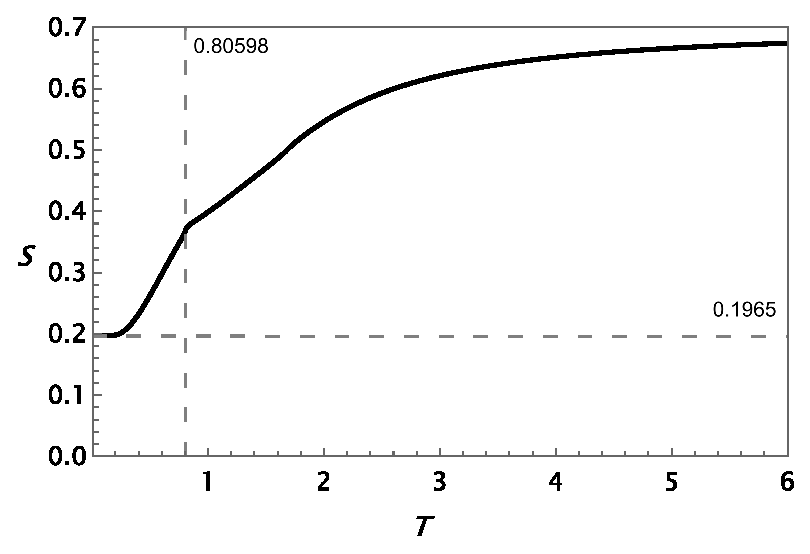
\includegraphics[width=1\linewidth]{part6/2transEnt2.eps} \\ б)}
	\end{minipage}
	\vfill
		\begin{minipage}{0.47\linewidth}
		\center{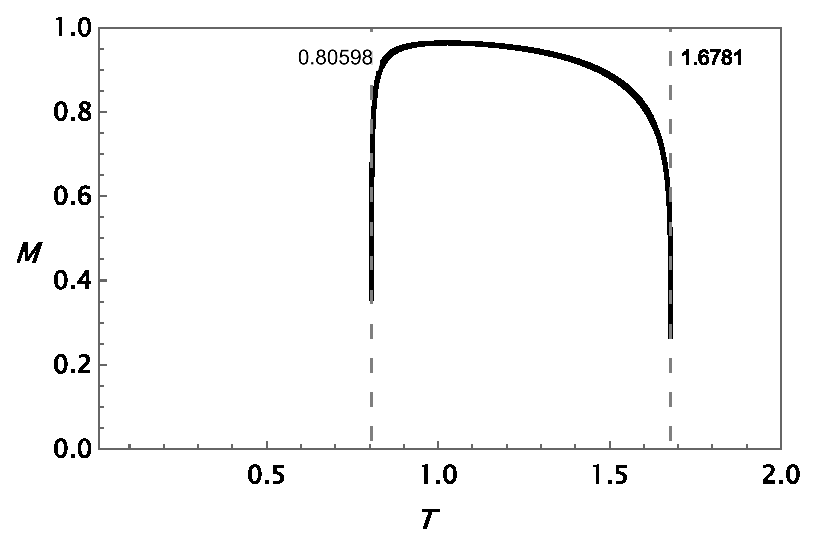
\includegraphics[width=1\linewidth]{part6/2transMag.eps} \\ в)}
	\end{minipage}
	\caption{а) Теплоемкость; б) энтропия и в) спонтанная намагниченность как функции температуры при $J_1 = 0.1, J_2 = -1.3, J_3 = -1.3, J_4 = -1.3, J_{d_1} = 1, J_{d_2} = 1, J_{d_3} = 1, J_{d_4} = 1$ и $d_1 = 4, d_2 = 4, d_3 = 4, d_4 = 4$}
	\label{2trans}
\end{figure}

Рисунок~\ref{3trans} демонстрирует систему уже с тремя фазовыми переходами при $J_1 = -1.27, J_2 = -1, J_3 = -1.27, J_4 = -1, J_{d_1} = 1.3, J_{d_2} = 1.3, J_{d_3} = 1.3, J_{d_4} = 1.3$ и $d_1 = 7, d_2 = 7, d_3 = 7, d_4 = 7$. На рисунках~\ref{3trans}а и~\ref{3trans}б можно увидеть теплоемкость с тремя фазовыми переходами $T_{N_1} \approx 0.25, T_{N_2} \approx 0.33736$ и $T_{N_3} \approx 2.5503$. 
Спонтанная намагниченность для данных параметров показана на рисунке~\ref{3trans}г. Здесь спонтанная намагниченность при $T \rightarrow 0$ максимальна и при дальнейшем увеличении температуры начинает падать и при значении $T_{N_1}$ полностью пропадает. После этого, в интервале температур от $T_{N_1}$ до $T_{N_2}$ полностью отсутствует. Начиная от $T_{N_2}$, появляется, достигая максимума, после чего снова падает. И уже при $T_{N_3}$ снова полностью исчезает. Данное явление в физике известно как явление реентерабельности~\cite{vaks1966}. 

 \begin{figure}[h]
	\begin{minipage}{0.47\linewidth}
		\center{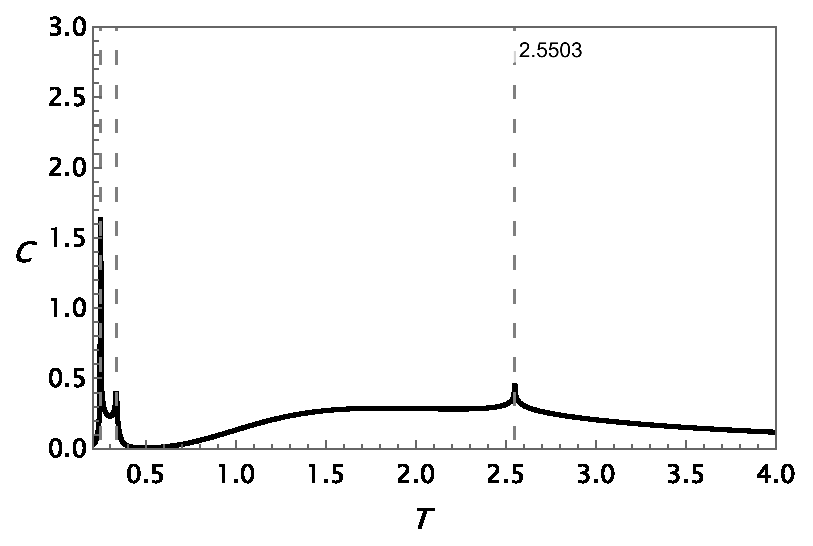
\includegraphics[width=1\linewidth]{part6/3transCapAll.eps} \\ а)}
	\end{minipage}
	\hfill
	\begin{minipage}{0.47\linewidth}
		\center{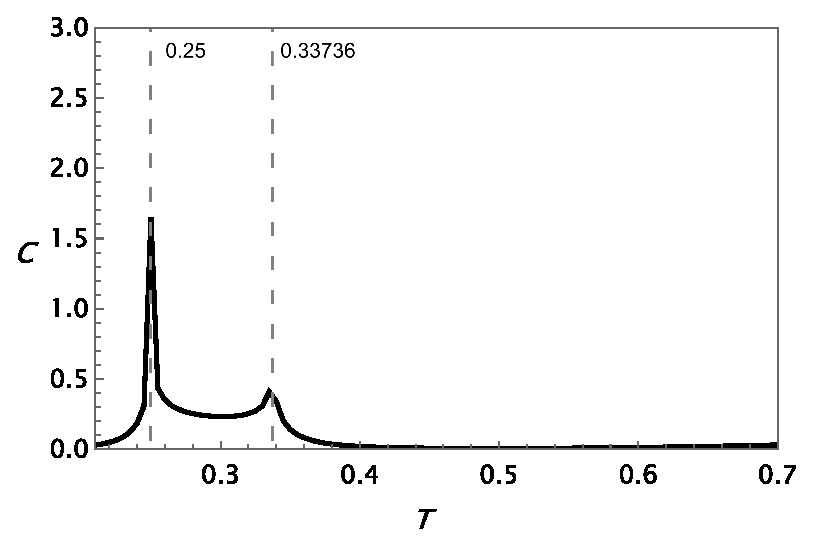
\includegraphics[width=1\linewidth]{part6/3transCapPart.eps} \\ б)}
	\end{minipage}
	\vfill
	\begin{minipage}{0.47\linewidth}
		\center{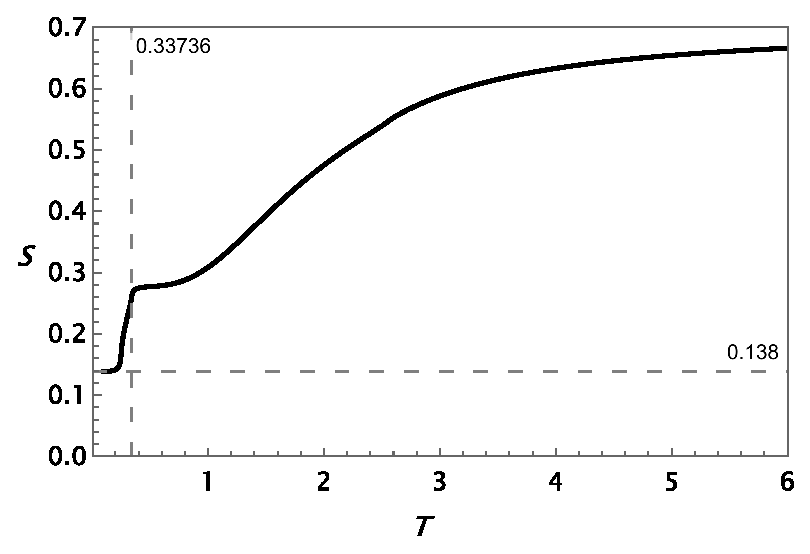
\includegraphics[width=1\linewidth]{part6/3transEnt.eps} \\ в)}
	\end{minipage}
	\hfill
	\begin{minipage}{0.47\linewidth}
		\center{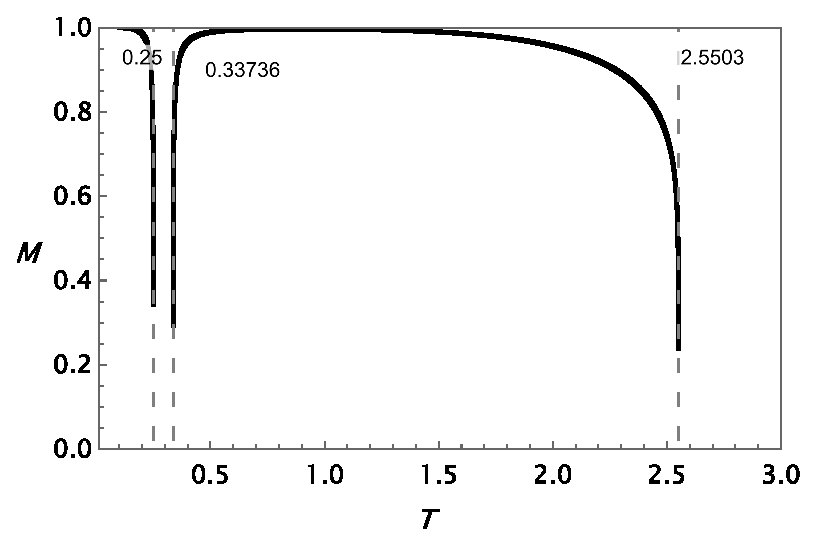
\includegraphics[width=1\linewidth]{part6/3transMag.eps} \\ г)}
	\end{minipage}
	\caption{а) Теплоемкость в диапазоне от $T=0.01$ до $T=4$; б) теплоемкость в диапазоне от $T=0.01$ до $T=0.7$; в) энтропия и г) спонтанная намагниченность как функции температуры при $J_1 = -1.27, J_2 = -1, J_3 = -1.27, J_4 = -1, J_{d_1} = 1.3, J_{d_2} = 1.3, J_{d_3} = 1.3, J_{d_4} = 1.3$ и $d_1 = 7, d_2 = 7, d_3 = 7, d_4 = 7$}
	\label{3trans}
\end{figure}

В заключение, рассмотрим систему сразу с пятью фазовыми переходами~(рис.~\ref{5trans}). Данная конфигурация получается, если выбрать обменные взаимодействия как $J_1 = -0.48621, J_2 = -1, J_3 = -0.671, J_4 = -1, J_{d_1} = 1.3, J_{d_2} = 1.3, J_{d_3} = 1.3, J_{d_4} = 1.3$ и степени декорирования как $d_1 = 7, d_2 = 7, d_3 = 7, d_4 = 7$. 

 \begin{figure}[h]
	\begin{minipage}{0.47\linewidth}
		\center{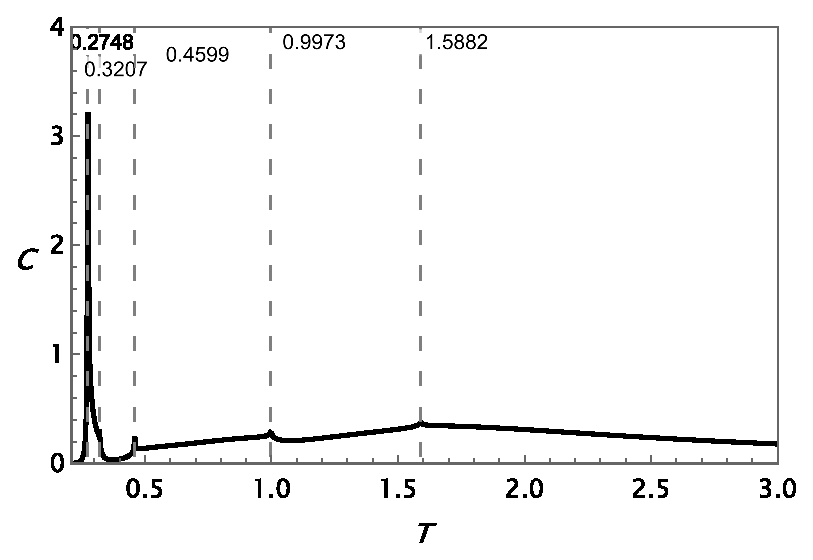
\includegraphics[width=1\linewidth]{part6/5transCapAll.eps} \\ а)}
	\end{minipage}
	\hfill
	\begin{minipage}{0.47\linewidth}
		\center{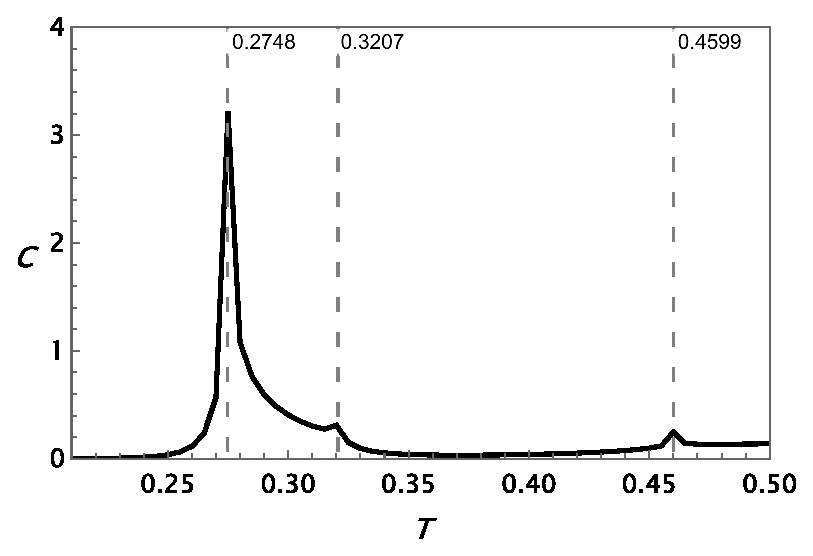
\includegraphics[width=1\linewidth]{part6/5transCapPart.eps} \\ б)}
	\end{minipage}
		\vfill
	\begin{minipage}{0.47\linewidth}
		\center{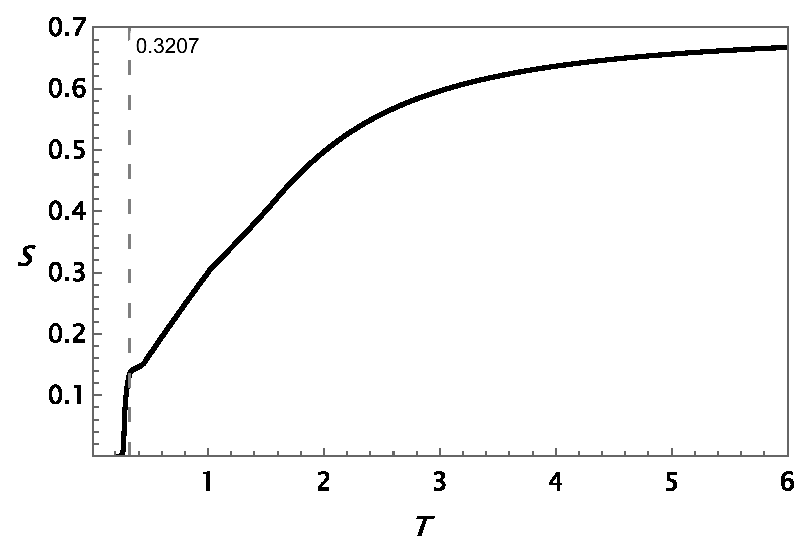
\includegraphics[width=1\linewidth]{part6/5transEnt.eps} \\ в)}
	\end{minipage}
	\hfill
	\begin{minipage}{0.47\linewidth}
		\center{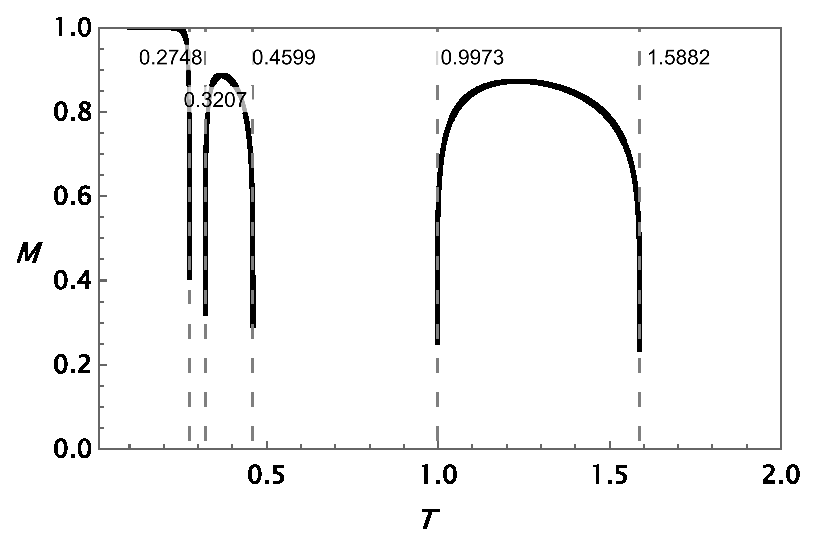
\includegraphics[width=1\linewidth]{part6/5transMag.eps} \\ г)}
	\end{minipage}
	\caption{а) Теплоемкость в диапазоне от $T=0.01$ до $T=3$; б) теплоемкость в диапазоне от $T=0.01$ до $T=0.5$; в) энтропия и г) спонтанная намагниченность как функции температуры при $J_1 = -0.48621, J_2 = -1, J_3 = -0.671, J_4 = -1, J_{d_1} = 1.3, J_{d_2} = 1.3, J_{d_3} = 1.3, J_{d_4} = 1.3$ и $d_1 = 7, d_2 = 7, d_3 = 7, d_4 = 7$}
	\label{5trans}
\end{figure}

В системе присутствуют 5 фазовых переходов при температурах $T_{N_1} \approx 0.2748$, $T_{N_2} \approx 0.3207$, $T_{N_3} \approx 0.4599$, $T_{N_4} \approx 0.9973$ и $T_{N_5} \approx 1.5882$ (см.~рис.~\ref{5trans}а и~рис.~\ref{5trans}б). Спонтанная намагниченность~\ref{5trans}г максимальна при низких температурах. С возрастанием температуры спонтанная намагниченность убывает и достигает нуля при $T_{N_1}$. Далее, спонтанная намагниченность отсутствует в интервале температур от $T_{N_1}$ до $T_{N_2}$, после чего вновь появляется от $T_{N_2}$ до $T_{N_3}$. Затем снова отсутствует в интервале температур от $T_{N_3}$ до $T_{N_4}$. При дальнейшем увеличении температуры от $T_{N_4}$ до $T_{N_5}$ возникает вновь. И полностью исчезает от температуры $T_{N_5}$, что соответствует состоянию парамагнетика. 

\section{Выводы по главе}

Выведено точное выражение для свободной энергии обобщенной модели Изинга с двумя трансляциями с учетом декорирования.

Выведено точное выражение для спонтанной намагниченности обобщенной модели Изинга с двумя трансляциями с учетом декорирования.

Исследованы термодинамические и фрустрационные свойства обобщенной модели Изинга с двумя трансляциями с учетом декорирования.

\FloatBarrier